\documentclass{article}

\usepackage[preprint]{corl_2026}

\usepackage[utf8]{inputenc}
\usepackage[T1]{fontenc}
\usepackage{amsmath,amssymb,bm}
\usepackage{booktabs}
\usepackage{graphicx}
\usepackage{tikz}
\usetikzlibrary{arrows.meta,positioning,calc,fit,backgrounds}
\usepackage{listings}
\usepackage{xcolor}
\usepackage{microtype}
\usepackage{float}
\usepackage{url}
\usepackage{enumitem}

% ---------- notation and helpers shared by both layouts ----------
\newcommand{\code}[1]{\texttt{#1}}
\newcommand{\subl}[1]{{\scriptsize\color{black!60}#1}}
\definecolor{series1}{HTML}{2A78D6}
\definecolor{series2}{HTML}{EB6834}
\definecolor{band}{HTML}{E7EEF1}
\definecolor{codebg}{HTML}{F4F5F4}
\definecolor{stagefill}{HTML}{DFEAEF}
\definecolor{stageline}{HTML}{1F6F8B}
\lstset{
  language=Python,
  commentstyle=\color{black!55}\itshape,
  keywordstyle=\bfseries,
  stringstyle=\color{black!70},
  backgroundcolor=\color{codebg},
  frame=single, framerule=0pt, framesep=3pt,
  columns=fullflexible, keepspaces=true,
  breaklines=true, breakatwhitespace=false, showstringspaces=false,
  numbers=left, numberstyle=\tiny\color{black!45}\ttfamily, numbersep=5pt, stepnumber=1,
  xleftmargin=18pt, xrightmargin=2pt,
  aboveskip=1pt, belowskip=0pt,
  literate={ö}{{\"o}}1 {ä}{{\"a}}1 {·}{{$\cdot$}}1 {—}{{--}}1 {→}{{$\to$}}1,
}
% file header above a listing: path on the left, line range on the right
\newcommand{\snippethead}[2]{\par\noindent{\scriptsize\sffamily\color{black!60}\path{#1}\hfill\mbox{#2}}\par\nopagebreak\vspace{-2pt}}
\newcommand{\snippetelide}{\par\nopagebreak\vspace{-5pt}\noindent{\scriptsize\color{black!45}\ttfamily\hspace{6pt}$\vdots$}\par\nopagebreak\vspace{-6pt}}
\tikzset{
  blk/.style={draw=black!55, rounded corners=2pt, minimum height=8mm, align=center, font=\small, inner sep=3pt, fill=black!4},
  stage/.style={blk, fill=stagefill, draw=stageline, line width=0.8pt},
  sub/.style={font=\scriptsize\color{black!60}},
  arr/.style={-{Latex[length=2mm]}, thick, black!70},
  darr/.style={-{Latex[length=2mm]}, thick, dashed, black!55},
}
% a snippet (header + listing, possibly with elisions). The optional argument is the number of text lines that
% must still fit on the page before the snippet may start, so the header always stays with the first code lines;
% a long listing may then break across pages instead of leaving a large gap at the page bottom.
\newenvironment{snippetbox}[1][8]{\par\addvspace{4pt}\penalty0
  \ifdim\pagegoal=\maxdimen\else
    \ifdim\dimexpr\pagegoal-\pagetotal\relax<#1\baselineskip \newpage\fi
  \fi
  \lstset{aboveskip=1pt, belowskip=0pt}}{\par\addvspace{4pt}}

\lstset{basicstyle=\ttfamily\scriptsize}

% colours of the HTML note, so the two renderings match
\definecolor{accent}{HTML}{1E6B86}
\definecolor{accentsoft}{HTML}{E2EEF2}
\definecolor{warnsoft}{HTML}{F6ECDC}
\definecolor{warn}{HTML}{8A5A12}

% figure and table wrappers: placed exactly where they are referenced (no floating)
\newenvironment{myfigure}{\begin{figure}[H]\centering}{\end{figure}}
\newenvironment{mytable}{\begin{table}[H]\centering}{\end{table}}
\newcommand{\myfigcaption}[2]{\caption{#2}\label{#1}}
\newcommand{\mytabcaption}[2]{\caption{#2}\label{#1}}

\title{How the Collision Check Sees the Robot:\\ Colliders, Point Clouds and a Phantom Hand in OmniReset}

\author{
  Tri Wahyu Guntara\\
  Tutorial notes on the UWLab OmniReset code base\\
}

\raggedbottom

\begin{document}
\maketitle

%==============================================================================
\section{Why the Success Test Looks for Collisions}
\label{sec:why}

Every reset state that the recorder writes to disk will one day be the first frame of a training episode~\cite{omnireset2026}. The policy starts there and physics takes over. If the hand in that frame already overlaps the peg by a few millimetres, the very first physics step pushes the two apart, the peg jumps, and the episode begins with a kick that the policy never asked for. If the fingers overlap the hole block, the kick can throw the arm. A library of such states teaches the policy that the world is jumpy and unfair, which is not what we want it to learn.

Physics itself does not forbid these overlaps. A rigid-body simulator tolerates small interpenetrations and resolves them over a step or two, which is why a hold can look perfectly calm in the viewport while the fingers sit a millimetre inside the peg. The success test therefore does its own measurement at the end of a hold. It asks, for each pair that matters, how deep the closest point of one body sits inside the other, and it compares that depth with the small allowance of Table~\ref{tab:allowances}.

\begin{mytable}
\small
\begin{tabular}{@{}p{0.30\linewidth}p{0.14\linewidth}p{0.50\linewidth}@{}}
\toprule
Pair & Allowed penetration & Why that number \\
\midrule
robot against the insertive object & 0.5 mm & Fingers that hold a peg touch it, and the solver leaves them a hair inside. Half a millimetre is contact, not a crash. \\
robot against the receptive object & 0 & The hand has no business touching the hole block in a recorded state. \\
insertive against receptive object & 1 mm & A partially inserted peg rests on the hole's wall. One millimetre is a resting contact under the solver's tolerance. \\
\bottomrule
\end{tabular}
\mytabcaption{tab:allowances}{The three penetration allowances of the reset-state success test.}
\end{mytable}

The code that performs this measurement is the \emph{collision analyzer}, one instance per row of the table, created by \code{check\_reset\_state\_success} in \code{mdp/terminations.py}. The rest of this note explains what it measures, how it measures it, and the mistake that was hiding in the first step.

%==============================================================================
\section{Bodies, Colliders and Prims}
\label{sec:prims}

Three words come up constantly, and they are easy to mix up.

\begin{description}[leftmargin=1.6em, style=nextline]
\item[Body] A rigid body is a piece of the world that moves as one unit. The peg is one body. The robot is many bodies, one per link, joined by joints. A body has a pose, which is a position and an orientation, and physics updates that pose every step.
\item[Collider] A collider is the shape physics uses to decide whether two bodies touch. It is attached to a body and moves with it. A collider is usually simpler than what you see on screen. The peg you see is a textured box, and its collider is a box of eight corners. The hole block's collider is a mesh of 2\,444 vertices, because a hole cannot be approximated by anything simpler. A body can carry several colliders, and the Dex1 base link carries a convex hull for its housing.
\item[Prim] A prim is a node in the USD scene file. Everything in the scene is a prim, arranged in a tree with paths that look like directories, for example \path{/World/envs/env_0/Robot/right_elbow_link}. A prim becomes a body when the file applies the \code{RigidBodyAPI} to it, and a prim becomes a collider when the file applies the \code{CollisionAPI} to it. The two labels are independent, and a collider prim normally sits somewhere below its body prim in the tree.
\end{description}

The last point is the one to hold on to, and Figure~\ref{fig:prims} draws it for the peg. Physics does not care how deep a collider prim sits below its body in the tree. It walks up from the collider until it meets a prim with the \code{RigidBodyAPI}, and that body owns the collider. Any code that reads the tree itself has to use the same rule, and we will see in Section~\ref{sec:phantom} what happens when it does not.

\begin{myfigure}
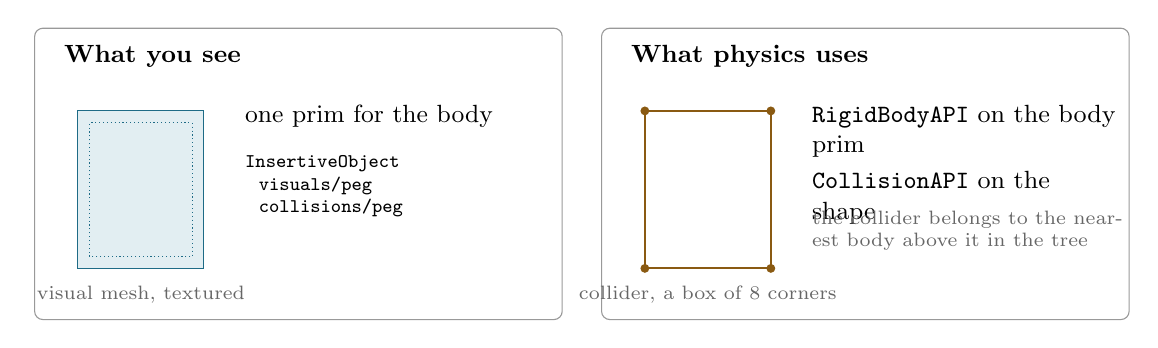
\begin{tikzpicture}[x=1cm, y=1cm, font=\small]
  % left panel
  \draw[rounded corners=3pt, black!40] (0,0) rectangle (6.7,3.7);
  \node[anchor=west, font=\small\bfseries] at (0.25,3.35) {What you see};
  \fill[accentsoft] (0.55,0.65) rectangle (2.15,2.65);
  \draw[accent] (0.55,0.65) rectangle (2.15,2.65);
  \draw[accent, densely dotted, thin] (0.7,0.8) rectangle (2.0,2.5);
  \node[sub, anchor=north] at (1.35,0.55) {visual mesh, textured};
  \node[anchor=north west, text width=3.9cm] at (2.55,2.85) {one prim for the body};
  \node[anchor=north west, font=\ttfamily\scriptsize, text width=3.9cm] at (2.55,2.2) {InsertiveObject\\ \ \ visuals/peg\\ \ \ collisions/peg};
  % right panel
  \begin{scope}[xshift=7.2cm]
  \draw[rounded corners=3pt, black!40] (0,0) rectangle (6.7,3.7);
  \node[anchor=west, font=\small\bfseries] at (0.25,3.35) {What physics uses};
  \draw[warn, thick] (0.55,0.65) rectangle (2.15,2.65);
  \foreach \p in {(0.55,0.65),(2.15,0.65),(0.55,2.65),(2.15,2.65)} \fill[warn] \p circle (1.6pt);
  \node[sub, anchor=north] at (1.35,0.55) {collider, a box of 8 corners};
  \node[anchor=north west, text width=3.9cm] at (2.55,2.85) {\code{RigidBodyAPI} on the body prim\\[2pt] \code{CollisionAPI} on the shape};
  \node[anchor=north west, sub, text width=3.9cm] at (2.55,1.5) {the collider belongs to the nearest body above it in the tree};
  \end{scope}
\end{tikzpicture}
\myfigcaption{fig:prims}{The peg as a prim tree. The visual mesh is what the renderer draws and the collider is what physics touches. Both sit below the body prim, and the collider is owned by that body because it is the nearest prim above it that carries the \code{RigidBodyAPI}.}
\end{myfigure}

%==============================================================================
\section{Measuring a Distance to a Mesh}
\label{sec:measure}

How far is the hand from the peg? The honest answer involves two complicated shapes, so the analyzer simplifies one side. It scatters sample points over the surface of the robot's colliders and measures each point against the object's mesh. The smallest value over all points is the answer.

\paragraph{Step 1, sample the robot.} When the environment starts, the analyzer picks 1\,024 points on the surface of each robot link it has been told to watch, spread evenly by farthest-point sampling so that no part of the link is missed. For the G1-D that list is the three shoulder links, the elbow, the three wrist links and the three Dex1 links, ten links and 10\,240 points. The points are stored once, in the link's own frame, because the link's shape never changes.

\paragraph{Step 2, move the points to where the link is now.} At the end of a hold the analyzer reads each link's current pose and carries the stored points along. A point $\mathbf{q}^{\ell}$ stored in the frame of link $\ell$ appears in the world at
\begin{equation}
  \mathbf{q}^{w} = \mathbf{R}_{\ell}\,\mathbf{q}^{\ell} + \mathbf{t}_{\ell},
  \label{eq:ride}
\end{equation}
where $\mathbf{R}_{\ell}$ and $\mathbf{t}_{\ell}$ are the link's rotation and position. The object has a pose too, so the point is then expressed in the object's frame, $\mathbf{q}^{o} = \mathbf{R}_{o}^{\top}(\mathbf{q}^{w} - \mathbf{t}_{o})$, which lets the object's mesh stay where it was loaded.

\paragraph{Step 3, ask the mesh.} Each point is handed to a Warp~\cite{macklin2022warp} mesh query, which returns the closest point $\mathbf{c}$ on the mesh surface and a sign $s$ that is $+1$ when the query point lies outside the solid and $-1$ when it lies inside. The signed distance is
\begin{equation}
  d(\mathbf{q}) = s\,\lVert \mathbf{q} - \mathbf{c} \rVert,
  \label{eq:sd}
\end{equation}
positive for a gap and negative for a penetration. The analyzer keeps the minimum over all points of all watched links, and the pair passes when
\begin{equation}
  \min_i d(\mathbf{q}_i) \;\ge\; d_{\min},
  \label{eq:pass}
\end{equation}
with $d_{\min}$ the allowance of Table~\ref{tab:allowances}. The query is limited to a radius $d_{\max}$ of 0.5~m. A point with no mesh within that radius returns no closest point, and the analyzer records $+0.5$ for it, meaning ``nothing anywhere near''. Figure~\ref{fig:points} shows the measurement on a finger pad, and the Warp kernel below is Equation~\eqref{eq:sd} line by line, with the scale of the collider undone before the length is taken.

\begin{snippetbox}[12]
\snippethead{source/uwlab_tasks/uwlab_tasks/manager_based/manipulation/omnireset/mdp/utils.py}{lines 293--306}
\begin{lstlisting}[firstnumber=293]
            mp = wp.mesh_query_point(mid, q3, max_dist)
            if mp.result:
                if check_dist:
                    closest = wp.mesh_eval_position(mid, mp.face, mp.u, mp.v)
                    local_dist = q3 - closest
                    unscaled_local_dist = wp.vec3(local_dist.x * crs.x, local_dist.y * crs.y, local_dist.z * crs.z)
                    delta_root = wp.quat_rotate(coll_rel_quat[index], unscaled_local_dist)
                    dist = wp.length(delta_root)
                    signed_dist = dist * mp.sign
                else:
                    signed_dist = mp.sign
                if signed_dist < best_signed_dist:
                    best_signed_dist = signed_dist
    signs[tid] = best_signed_dist
\end{lstlisting}
\end{snippetbox}


\begin{myfigure}
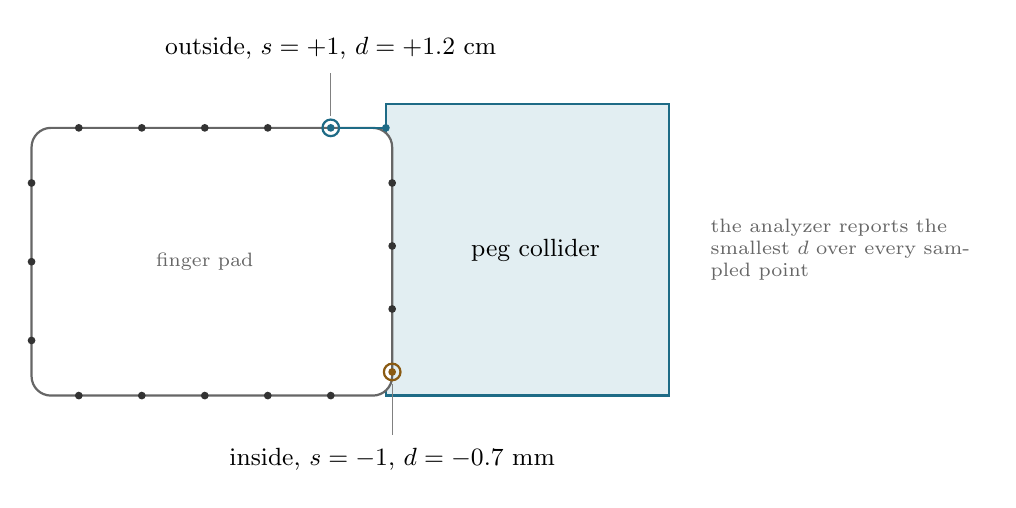
\begin{tikzpicture}[x=1cm, y=1cm, font=\small]
  % the peg's collider, and the finger pad pressed a little into its left face
  \fill[accentsoft] (5.7,0.9) rectangle (9.3,4.6);
  \draw[accent, thick] (5.7,0.9) rectangle (9.3,4.6);
  \node at (7.6,2.75) {peg collider};
  \draw[rounded corners=7pt, black!60, thick, fill=white] (1.2,0.9) rectangle (5.78,4.3);
  \node[sub] at (3.4,2.6) {finger pad};
  % sample points on the pad's surface
  \foreach \p in {(1.8,4.3),(2.6,4.3),(3.4,4.3),(4.2,4.3),(1.2,3.6),(1.2,2.6),(1.2,1.6),(1.8,0.9),(2.6,0.9),(3.4,0.9),(4.2,0.9),(5.0,0.9),(5.78,3.6),(5.78,2.8),(5.78,2.0)} \fill[black!80] \p circle (1.4pt);
  % a point on the top edge, outside: its closest surface point is straight across on the peg's face
  \fill[accent] (5.0,4.3) circle (1.4pt);
  \draw[accent, thick] (5.0,4.3) circle (3pt);
  \draw[accent, thick] (5.11,4.3) -- (5.7,4.3);
  \fill[accent] (5.7,4.3) circle (1.4pt);
  \draw[black!50] (5.0,4.45) -- (5.0,5.0);
  \node[anchor=south] at (5.0,5.05) {outside, $s=+1$, $d=+1.2$ cm};
  % a point on the pressed edge, inside the peg by less than a millimetre
  \fill[warn] (5.78,1.2) circle (1.4pt);
  \draw[warn, thick] (5.78,1.2) circle (3pt);
  \draw[black!50] (5.78,1.05) -- (5.78,0.4);
  \node[anchor=north] at (5.78,0.35) {inside, $s=-1$, $d=-0.7$ mm};
  % what the analyzer keeps
  \node[anchor=west, sub, text width=3.4cm] at (9.7,2.75) {the analyzer reports the smallest $d$ over every sampled point};
\end{tikzpicture}
\myfigcaption{fig:points}{Sample points on a finger pad beside the peg. For each point the mesh query finds the closest surface point and a sign. The pad is pressed a little into the peg, so one of its points lies inside and reports a negative distance. That smallest value is what the pair is judged on, here against the half-millimetre allowance.}
\end{myfigure}

\paragraph{The sign-only mode.} When an allowance is exactly zero, as for the robot against the hole block, the analyzer skips the length and keeps only the sign (\code{check\_dist} is false in the kernel above). Any point inside makes the pair report $-1$, and no point inside leaves it at $+0.5$. This is why a debug block shows \code{min\_signed\_dist=-1.00000} for that pair instead of a millimetre figure. It is a yes or no, not a depth. The verdict itself is one comparison:

\begin{snippetbox}[8]
\snippethead{source/uwlab_tasks/uwlab_tasks/manager_based/manipulation/omnireset/mdp/collision_analyzer.py}{lines 190--201}
\begin{lstlisting}[firstnumber=190]
        signs = (
            wp.to_torch(sign_w)
            .view(len(self.obstacles), len(env_ids), len(self.body_ids), self.cfg.num_points)
            .amin(dim=0)
        )
        # collision_points = cloud[(signs < 0.0)]
        # for i in range(500):
        #     env.sim.render()
        #     visualizer.visualize(collision_points.view(-1, 3))

        coll_free_mask = signs.amin(dim=(1, 2)) >= self.cfg.min_dist
        return coll_free_mask
\end{lstlisting}
\end{snippetbox}


%==============================================================================
\section{Points Ride on Their Own Link}
\label{sec:ride}

Step 2 contains an assumption that is easy to overlook. The stored points of a link are moved with that link's pose and nothing else. A point sampled on the fingertip must be stored in the fingertip's frame and moved with the fingertip. If it were stored in the elbow's frame and moved with the elbow, it would be correct only while the wrist stayed exactly as it was when the point was sampled, which is the rest pose of the robot file.

Write the fingertip's pose as the elbow's pose followed by the chain of wrist joints between them, $\mathbf{T}_{h} = \mathbf{T}_{e}\,\mathbf{T}_{e\to h}(\boldsymbol{\theta})$, where $\boldsymbol{\theta}$ holds the wrist angles. A fingertip point stored in the elbow frame at the rest pose and carried by the elbow lands at
\begin{equation}
  \mathbf{T}_{e}\,\mathbf{T}_{e\to h}(\boldsymbol{\theta}_0)\,\mathbf{q}^{h}
  \quad\text{instead of}\quad
  \mathbf{T}_{e}\,\mathbf{T}_{e\to h}(\boldsymbol{\theta})\,\mathbf{q}^{h}.
  \label{eq:phantom}
\end{equation}
The two agree only when $\boldsymbol{\theta} = \boldsymbol{\theta}_0$. Bend the wrist by sixty degrees and the stored copy of the fingertip stays on the straight line through the forearm, about twenty centimetres from the real one on the G1. The analyzer would then measure a fingertip that does not exist.

%==============================================================================
\section{The Phantom Hand}
\label{sec:phantom}

This is exactly what happened on the G1-D and the G1 with the Dex3, and the reason is how their files are laid out. The UR5e file lists its links side by side under the robot prim. The two G1 files were produced by the Kit URDF importer, which nests each link prim inside its parent link, so the tree follows the kinematic chain:

\begin{lstlisting}[language={}, numbers=none, xleftmargin=4pt, basicstyle=\ttfamily\scriptsize]
Robot
+- torso_link
   +- right_shoulder_pitch_link
      +- right_shoulder_roll_link
         +- right_shoulder_yaw_link
            +- right_elbow_link            <- body, with its own collider below it
               +- right_wrist_roll_link    <- also a body, and also below the elbow prim
                  +- right_wrist_pitch_link
                     +- right_wrist_yaw_link
                        +- right_dex1_base_link
                           +- right_dex1_finger_link_1
                           +- right_dex1_finger_link_2
\end{lstlisting}

The analyzer builds a link's point cloud by collecting every collider prim below that link's prim. On the UR5e that rule finds exactly the link's own colliders. On the G1 it finds the link's own collider and then every collider of every link further down the chain, because they all sit below the elbow prim in the tree. The elbow's cloud ends up containing the forearm, the wrist and the whole hand, all expressed in the elbow frame at the rest pose and all carried around rigidly by the elbow. The same happens one level down for each wrist link. Figure~\ref{fig:chain} shows the two rules side by side.

\begin{myfigure}
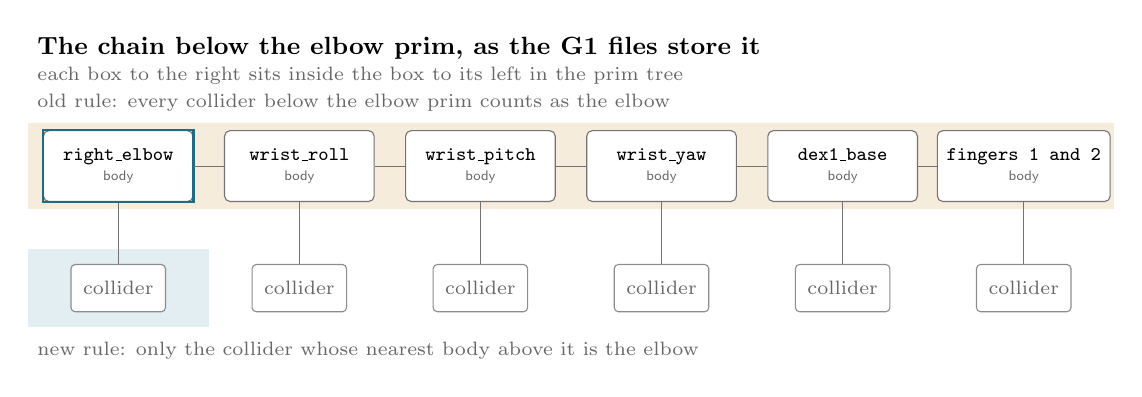
\begin{tikzpicture}[x=1cm, y=1cm, font=\small,
  body/.style={draw=black!55, rounded corners=2pt, fill=white, minimum width=19mm, minimum height=9mm, align=center, font=\scriptsize\ttfamily},
  col/.style={draw=black!45, rounded corners=1.5pt, fill=white, minimum width=12mm, minimum height=6mm, font=\scriptsize\color{black!60}}]
  \fill[warnsoft] (-0.2,1.45) rectangle (13.6,2.55);
  \node[anchor=west, sub] at (-0.2,2.8) {old rule: every collider below the elbow prim counts as the elbow};
  \fill[accentsoft] (-0.2,-0.05) rectangle (2.1,0.95);
  \node[anchor=west, sub] at (-0.2,-0.35) {new rule: only the collider whose nearest body above it is the elbow};
  \foreach \i/\name in {0/right\_elbow, 1/wrist\_roll, 2/wrist\_pitch, 3/wrist\_yaw, 4/dex1\_base, 5/{fingers 1 and 2}} {
    \node[body] (b\i) at ({0.95 + 2.3*\i}, 2.0) {\name\\[-1pt]{\tiny\sffamily\color{black!60}body}};
    \node[col] (c\i) at ({0.95 + 2.3*\i}, 0.45) {collider};
    \draw[black!55] (b\i) -- (c\i);
  }
  \draw[accent, thick] (b0.south west) rectangle (b0.north east);
  \foreach \i in {0,...,4} { \pgfmathtruncatemacro{\j}{\i+1} \draw[black!55] (b\i) -- (b\j); }
  \node[anchor=west, font=\small\bfseries] at (-0.2,3.5) {The chain below the elbow prim, as the G1 files store it};
  \node[anchor=west, sub] at (-0.2,3.15) {each box to the right sits inside the box to its left in the prim tree};
\end{tikzpicture}
\myfigcaption{fig:chain}{The elbow and everything the G1 files nest below it. The old rule took every collider in the upper band as part of the elbow. The new rule keeps the lower band, the one collider whose nearest body above it is the elbow itself.}
\end{myfigure}

How much of each cloud was phantom? Table~\ref{tab:share} gives the share of sampled collider area that belongs to descendant links, measured on the two robot files. It is large for every arm link.

\begin{mytable}
\small
\begin{tabular}{@{}lcc@{}}
\toprule
Link & G1-D with Dex1 & G1 with Dex3 \\
\midrule
right\_shoulder\_yaw\_link & 71\% & 71\% \\
right\_elbow\_link & 84\% & 83\% \\
right\_wrist\_roll\_link & 88\% & 88\% \\
right\_wrist\_pitch\_link & 83\% & 82\% \\
right\_wrist\_yaw\_link & 84\% & 83\% \\
gripper base or palm & 21\% & 45\% \\
Dex3 thumb\_1 & -- & 100\% \\
\bottomrule
\end{tabular}
\mytabcaption{tab:share}{Share of each link's sampled collider area that belongs to descendant links, before the fix.}
\end{mytable}

Five out of six points on the elbow's cloud were a frozen copy of the wrist and the hand. During a hold the real wrist is bent to put the hand on the peg, so these copies stick out of the elbow and the wrist links along the rest-pose direction, roughly where the hand would be if the arm were straight. They can land inside the hole block, inside the peg or under the table, and the analyzer reports a collision that no one can see in the viewport. Figure~\ref{fig:arm} draws the situation.

\begin{myfigure}
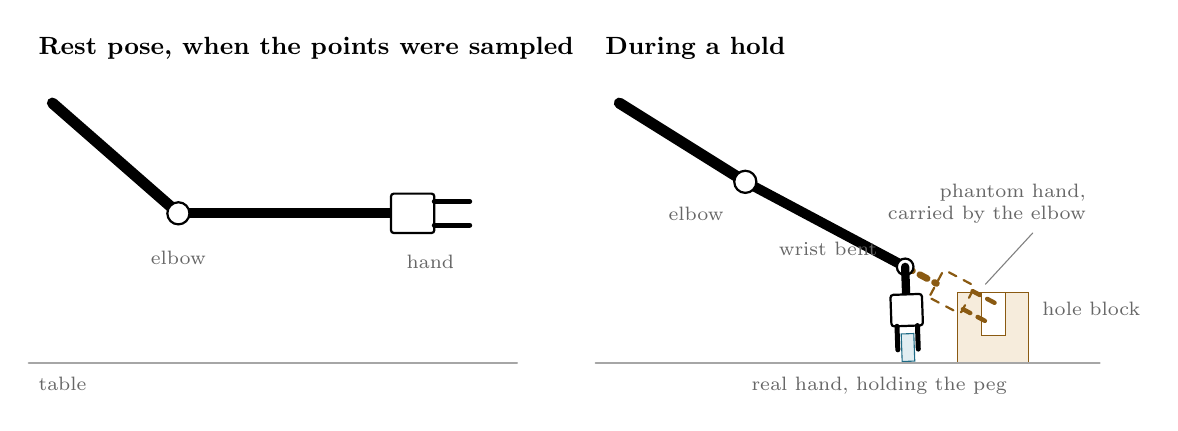
\begin{tikzpicture}[x=1cm, y=1cm, font=\small, line cap=round]
  % left: rest pose
  \node[anchor=west, font=\small\bfseries] at (0,4.3) {Rest pose, when the points were sampled};
  \draw[line width=4pt] (0.3,3.6) -- (1.9,2.2);
  \draw[line width=3.6pt] (1.9,2.2) -- (4.6,2.2);
  \fill[white] (1.9,2.2) circle (4pt); \draw[thick] (1.9,2.2) circle (4pt);
  \node[sub, anchor=north] at (1.9,1.85) {elbow};
  \draw[thick, fill=white, rounded corners=1pt] (4.6,1.95) rectangle (5.15,2.45);
  \draw[line width=1.8pt] (5.15,2.35) -- (5.6,2.35);
  \draw[line width=1.8pt] (5.15,2.05) -- (5.6,2.05);
  \node[sub, anchor=north] at (5.1,1.8) {hand};
  \draw[black!35, thick] (0,0.3) -- (6.2,0.3);
  \node[sub, anchor=north west] at (0,0.25) {table};
  % right: during a hold. The forearm slopes down, the wrist bends the real hand onto the peg, and the phantom
  % copy continues along the forearm into the hole block.
  \begin{scope}[xshift=7.2cm]
  \node[anchor=west, font=\small\bfseries] at (0,4.3) {During a hold};
  \coordinate (E) at (1.9,2.6);
  \coordinate (W) at (3.93,1.52);
  \draw[line width=4pt] (0.3,3.6) -- (E);
  \draw[line width=3.6pt] (E) -- (W);
  \fill[white] (E) circle (4pt); \draw[thick] (E) circle (4pt);
  \node[sub, anchor=north east] at (1.75,2.4) {elbow};
  \fill[warnsoft] (4.6,0.3) rectangle (5.5,1.2); \draw[warn] (4.6,0.3) rectangle (5.5,1.2);
  \fill[white] (4.9,0.65) rectangle (5.2,1.2); \draw[warn, thin] (4.9,0.65) rectangle (5.2,1.2);
  \node[sub, anchor=north west] at (5.55,1.2) {hole block};
  \begin{scope}[shift={(W)}, rotate=-28]
    \draw[warn, line width=2.4pt, dashed] (0,0) -- (0.45,0);
    \draw[warn, thick, dashed, rounded corners=1pt] (0.45,-0.2) rectangle (0.9,0.2);
    \draw[warn, line width=1.6pt, dashed] (0.9,0.13) -- (1.3,0.13);
    \draw[warn, line width=1.6pt, dashed] (0.9,-0.13) -- (1.3,-0.13);
  \end{scope}
  \node[sub, anchor=south east, align=right] at (6.35,1.95) {phantom hand,\\carried by the elbow};
  \draw[black!50] (5.55,1.95) -- (4.95,1.3);
  \fill[white] (W) circle (3pt); \draw[thick] (W) circle (3pt);
  \node[sub, anchor=east] at (3.7,1.75) {wrist bent};
  \begin{scope}[shift={(W)}, rotate=-88]
    \draw[line width=3pt] (0,0) -- (0.35,0);
    \draw[thick, fill=white, rounded corners=1pt] (0.35,-0.2) rectangle (0.75,0.2);
    \draw[line width=1.8pt] (0.75,0.13) -- (1.05,0.13);
    \draw[line width=1.8pt] (0.75,-0.13) -- (1.05,-0.13);
    \fill[accentsoft] (0.85,-0.08) rectangle (1.2,0.08); \draw[accent] (0.85,-0.08) rectangle (1.2,0.08);
  \end{scope}
  \node[sub, anchor=north] at (3.6,0.25) {real hand, holding the peg};
  \draw[black!35, thick] (0,0.3) -- (6.4,0.3);
  \end{scope}
\end{tikzpicture}
\myfigcaption{fig:arm}{Left, the arm as the robot file stores it, which is when the point clouds are sampled. Right, the arm during a hold with the wrist bent down onto the peg. The real hand is where physics has it. The elbow's point cloud still carries a copy of the hand on the straight line through the forearm, drawn dashed, and that copy can sit inside the hole block or below the table while the real hand is nowhere near.}
\end{myfigure}

The debug block that exposed this contained a contradiction. The pair robot against the hole block reported $-1$, a point inside, while the pair peg against the hole block reported $+0.5$, nothing within half a metre. The peg was in the hand, eleven centimetres from the gripper frame, so the real hand was more than a third of a metre from the hole. Only a point that was not on the real hand could have been inside. Checking the hole mesh itself first ruled out the other suspects, since the mesh is watertight with consistent winding, and Warp's sign gave no false insides on 28\,000 test points around it.

%==============================================================================
\section{The Fix, and What It Changes}
\label{sec:fix}

The rule physics uses is the rule the sampler should use. A collider belongs to the nearest body above it in the tree. The hasher that collects colliders, \code{RigidObjectHasher} in \code{mdp/rigid\_object\_hasher.py}, now applies that rule whenever the prim it was asked about is itself a body. The call site filters the collected colliders before anything is counted or hashed:

\begin{snippetbox}[12]
\snippethead{source/uwlab_tasks/uwlab_tasks/manager_based/manipulation/omnireset/mdp/rigid_object_hasher.py}{lines 61--69}
\begin{lstlisting}[firstnumber=61]
            coll_prims = get_all_matching_child_prims(
                prim_paths[i],
                predicate=lambda p: p.GetTypeName() in ("Mesh", "Cube", "Sphere", "Cylinder", "Capsule", "Cone")
                and p.HasAPI(UsdPhysics.CollisionAPI),
                traverse_instance_prims=True,
            )
            root_prim = stage.GetPrimAtPath(prim_paths[i])
            coll_prims = self._own_colliders(root_prim, coll_prims)
            if len(coll_prims) == 0:
\end{lstlisting}
\end{snippetbox}


and the filter itself climbs from each collider until it meets a body:

\begin{snippetbox}[14]
\snippethead{source/uwlab_tasks/uwlab_tasks/manager_based/manipulation/omnireset/mdp/rigid_object_hasher.py}{lines 136--162}
\begin{lstlisting}[firstnumber=136]
    @staticmethod
    def _own_colliders(root_prim: Usd.Prim, coll_prims: list[Usd.Prim]) -> list[Usd.Prim]:
        """Drop the colliders that belong to another rigid body nested under ``root_prim``.

        A robot converted by the Kit URDF importer nests each link prim inside its parent link, so every
        collider of the forearm, the wrist and the hand also lies under the elbow prim. Sampled as part of the
        elbow they would be frozen at the rest pose and carried around with it. When the root is itself a rigid
        body, only the colliders whose nearest rigid-body ancestor is that root are kept. A root without the
        rigid-body API (an object wrapper prim) keeps every collider under it, as before.

        Args:
            root_prim: The prim the colliders were collected under.
            coll_prims: The colliders found under ``root_prim``.

        Returns:
            The colliders owned by ``root_prim`` itself.
        """
        if not root_prim.HasAPI(UsdPhysics.RigidBodyAPI):
            return coll_prims
        own = []
        for prim in coll_prims:
            parent = prim.GetParent()
            while parent.IsValid() and parent != root_prim and not parent.HasAPI(UsdPhysics.RigidBodyAPI):
                parent = parent.GetParent()
            if parent == root_prim:
                own.append(prim)
        return own
\end{lstlisting}
\end{snippetbox}


For the elbow, the climb from the wrist's collider meets the wrist body first, so that collider is dropped. The climb from the elbow's own collider meets the elbow, so it is kept. Objects are untouched, because their prim path points at a wrapper without the body label, and the UR5e is untouched because its tree was flat all along.

Three things follow from the change.
\begin{itemize}[leftmargin=1.4em]
  \item The robot analyzers on both G1 robots now measure the real arm. A collision reported by the success test is a collision you can find in the viewport.
  \item The grasp sampler's own collision filter used the same hasher on the Dex3 and Dex1 hand files, which nest the same way, so it was also judging phantom finger copies. Its yield and the depth of the recorded grasps are worth a second look.
  \item The success rates measured for the G1 reset-state families before the fix included rejections for phantom collisions. The funnel counts should be taken again.
\end{itemize}

A tell for the future: a link that reports many more colliders than it visibly has is the signature of this layout. The inspection that produced Table~\ref{tab:share} counts, for every body prim, the colliders whose nearest body is a different one. On a flat file every count is zero.

%==============================================================================
\section{Reading a Debug Block}
\label{sec:debug}

With \code{debug=True} on the success term, every hold that reaches its final step prints one block. Here is the block that started this investigation, from the in-air grasped family on the G1-D, read line by line.

\begin{lstlisting}[language={}, numbers=none, xleftmargin=4pt, basicstyle=\ttfamily\scriptsize]
[check_reset_state_success] env 0: success=False
  abnormal_gripper_state=False (any joint > 2x vel limit)
  gripper_orientation_within_range=False approach_z=-0.3401 (< -0.5)
  stability_reached=True counter=30/5
  excessive_pose_deviation=False
    InsertiveObject pos_deviation=0.0082 (<= 0.05)
    ReceptiveObject pos_deviation=0.0000 (<= 0.05)
    Robot pos_deviation=0.0020 (<= 0.1)
  pos_below_threshold=False min_pos_z=0.8702 (>= 0.835)
  collision_free=False
    robot-insertive_object min_signed_dist=-0.00027 (>= -0.0005)
    robot-receptive_object min_signed_dist=-1.00000 (>= 0.0)
    insertive_object-receptive_object min_signed_dist=0.50000 (>= -0.001)
  fingers_blocked=True open_fraction=[0.237, 0.292] mean=0.265 (0.08 < mean < 0.9)
  object_near_ee=True object_ee_dist=0.1075 (< 0.2)
  at_grasp_pose=True pos_err=0.0011 (< 0.015) ang_err=0.0021 (< 0.26)
\end{lstlisting}

\begin{description}[leftmargin=1.6em, style=nextline]
\item[abnormal\_gripper\_state] No joint of the robot moved faster than twice its velocity limit at the final step. A violent step would show here.
\item[gripper\_orientation\_within\_range] The Dex1's approach axis has a world $z$ component of $-0.34$, which is seventy degrees from pointing straight down. The rule asks for sixty degrees or less, so this clause failed. The hold itself was fine, and this rejection is a policy of the family, not a flaw in the grasp.
\item[stability\_reached] Everything was quiet for all thirty steps, well past the five required.
\item[excessive\_pose\_deviation and pos\_below\_threshold] The peg moved 8~mm since the reset, the hand 2~mm, the hole block not at all, and nothing dropped below two centimetres under the table top. All well inside their limits.
\item[collision\_free] The hand sits 0.27~mm inside the peg, which is ordinary contact and under the half-millimetre allowance. The hole block reports a point inside in the sign-only mode, and the peg reports nothing within half a metre of the block. That contradiction is Section~\ref{sec:phantom}.
\item[fingers\_blocked, object\_near\_ee, at\_grasp\_pose] The fingers stopped at a quarter of their travel, so something is between them. The peg is 11~cm from the gripper frame. The hand is 1~mm and 0.1 degrees from the dataset's grasp pose. These three together say the peg is held exactly as sampled.
\end{description}

So this block describes a real grasp that failed for one legitimate reason, its approach angle, and one phantom reason, a collider copy inside the hole block. After the fix only the first remains, and whether a seventy-degree approach should count as a valid in-air state is a question about the family, not about the analyzer.

%==============================================================================
\section{Check Your Understanding}
\label{sec:check}

\begin{enumerate}[leftmargin=1.6em]
  \item The peg analyzer reports $+0.5$ and the robot analyzer reports $-1$. Why can both not be true at once for a hand that holds the peg?

  \emph{Answer.} $+0.5$ means no point of the peg has any hole-block mesh within half a metre. The hand is within about eleven centimetres of the peg, so no point on the real hand can be inside the block. A $-1$ must then come from a point that is not on the real hand.
  \item Why does the fix not change anything for the peg or the hole block?

  \emph{Answer.} Their prim paths point at a wrapper prim without the \code{RigidBodyAPI}. The new rule only applies when the queried prim is itself a body, so for objects every collider below the wrapper is kept, as before.
  \item Why did the UR5e never show the problem?

  \emph{Answer.} Its file lists the links side by side under the robot prim. No link prim contains another link, so collecting every collider below a link already gives only that link's own colliders.
  \item A hold shows \code{robot-insertive\_object min\_signed\_dist=-0.0009}. Is that a crash?

  \emph{Answer.} It is a 0.9~mm penetration, which fails the 0.5~mm allowance, but it is the kind of depth a soft fingertip pressed on a peg reaches when the solver settles. It says the grasp is squeezing hard rather than that the hand is passing through the peg. Whether to loosen the allowance is a judgement about how the fingers are driven.
\end{enumerate}

\paragraph{Files involved.} \path{mdp/collision_analyzer.py}, \path{mdp/rigid_object_hasher.py}, \path{mdp/utils.py} (\code{sample\_object\_point\_cloud}, \code{get\_signed\_distance}) and \path{mdp/terminations.py}. The measurements come from the robot USD files under \path{source/uwlab_assets/data/Robots/Unitree}. Written 30 October 2026 for the \code{feature/forge-omnireset} branch.


\bibliography{references}

\end{document}
